\chapter{Arhitektura i dizajn sustava}
		
		\textbf{\textit{dio 1. revizije}}\\

		\textit{ Potrebno je opisati stil arhitekture te identificirati: podsustave, preslikavanje na radnu platformu, spremišta podataka, mrežne protokole, globalni upravljački tok i sklopovsko-programske zahtjeve. Po točkama razraditi i popratiti odgovarajućim skicama:}
	\begin{itemize}
		\item 	\textit{izbor arhitekture temeljem principa oblikovanja pokazanih na predavanjima (objasniti zašto ste baš odabrali takvu arhitekturu)}
		\item 	\textit{organizaciju sustava s najviše razine apstrakcije (npr. klijent-poslužitelj, baza podataka, datotečni sustav, grafičko sučelje)}
		\item 	\textit{organizaciju aplikacije (npr. slojevi frontend i backend, MVC arhitektura) }		
	\end{itemize}
	
		Arhitektura se može podijeliti na nekoliko podsustava:
		 \begin{itemize}
			\item Poslužitelj frontenda
			\item Frontend (prvi dio web aplikacije)
			\item Poslužitelj backenda
			\item Backend (drugi dio web aplikacije)
			\item Baza podataka 
		\end{itemize}
		
		\begin{figure}[H]
			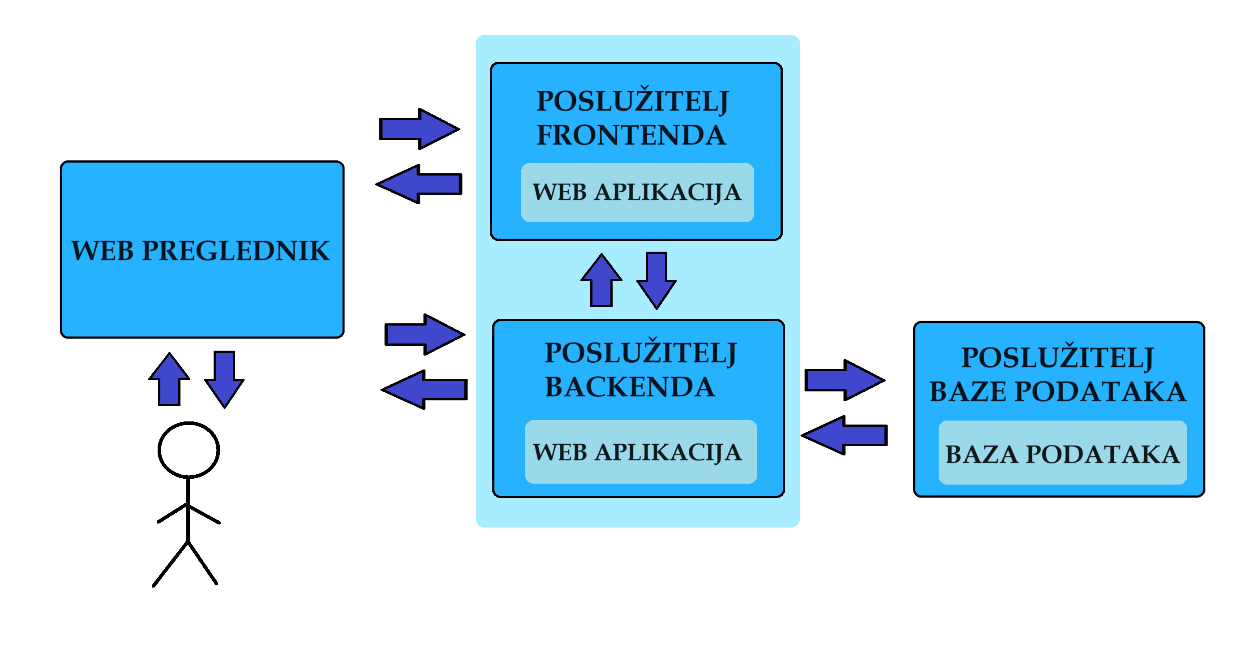
\includegraphics[width=\textwidth]{slike/arhitekturaSustava.PNG} %veličina u odnosu na širinu linije
			\caption{Arhitektura sustava}
			\label{fig:promjene9} %label mora biti drugaciji za svaku sliku
		\end{figure}
		
		 \underbar{\textit{Web preglednik}} je program koji omogućuje korisnicima pregled web sadržaja, a to uključuje web stranice i njihov raznolik sadržaj (slike, dijagrami...). Web preglednik je i okolina u kojoj se mogu izvršiti skripte (potrebno npr. kod client-side renderinga). Jedna od glavnih funkcionalnosti web preglednika je slanje zahtjeva prema web poslužiteljima.
		 	
		 \underbar{\textit{Frontend poslužitelj}} je poslužitelj koji komunicira s web preglednikom klijenta preko HTTP (\textit{engl. Hyper Text Transfer Protocol}) protokola. Na frontend poslužitelju se nalazi frontend dio web aplikacije čije dijelove frontend poslužitelj vraća klijentu na zahtjev (npr. pri početnom otvaranju stranice).
		 
		 \underbar{\textit{Backend poslužitelj}} je poslužitelj na kojem se nalazi backend dio aplikacije. Backend poslužitelj omogućuje slanje i primanje zahtjeva backend dijelu aplikacije. Backend poslužitelj preko HTTP protokola komunicira s frontendom ili web preglednikom klijenta. Ovaj poslužitelj komunicira i s poslužiteljem baze podataka preko TCP (eng. Transmission Control Protocol) protokola.
		 
		 \underbar{\textit{Web aplikacija}} dijeli se na frontend i backend. Zadaća frontend dijela je oblikovanje prikaza podataka, a potrebne podatke može zatražiti od backenda. Zadaća backend dijela je dohvaćanje podataka iz baze te njihova obrada i prosljeđivanje frontendu u određenom obliku. Komunikacija između frontenda, backenda, baze i web preglednika odvija se preko zahtjeva.
		 
		 \underbar{\textit{Baza podataka}} sadrži sve informacije o korisničkim računima, korisnicima te porukama koje korisnici šalju unutar web aplikacije.\\
		 	
		 Razvojni okvir koji smo odabrali za razvijanje backend dijela aplikacije jest Spring (programski jezik Java). Za razvoj frontend dijela aplikacije odlučili smo se za razvojni okvir React (programski jezik JavaScript). Odabrano razvojno okruženje je IntelliJ IDEA. Baza podataka napravljena je koristeći PostgreSQL.\\
		 
		 Arhitektura web aplikacije temelji se na single-page application principu kojeg omogućuje razvojni okvir React. Pri početnom otvaranju web aplikacije, web preglednik korisnika uputi zahtjev frontend serveru koji mu vraća sve odgovarajuće datoteke potrebne za prikaz stranice u pregledniku (koristi se princip client-side rendering). Ovisno o prosljeđenim podacima, web preglednik prilikom obrađivanja ulaznih podataka korisnika (klik na pojedini gumb, otvaranje nove stranice) šalje zahtjeve backend serveru (ako su potrebni određeni podaci za prikaz React komponente) ili frontend serveru (za dohvat datoteka potrebnih za prikaz novog dijela stranice).
		 
		  	
		  

	
		

		

				
		\section{Baza podataka}
			
			\textbf{\textit{dio 1. revizije}}\\
			
		\textit{Potrebno je opisati koju vrstu i implementaciju baze podataka ste odabrali, glavne komponente od kojih se sastoji i slično.}
		
		Za našu web aplikaciju koristiti ćemo relacijsku bazu podataka koja je industrijski standard te najjednostavniji način za rješenje našeg problema. Osnovni element baze je relacija čija su obilježja njeno ime i atributi. Glavna zadaća naše baze je spajanje njenih korisnika i sustava s korisnikom, bilo kroz poruke ili kroz razne obrasce.
		Entitet ove baze podataka su:
		
			\begin{packed_item}
				\item Roditelj
				\item Dijete
				\item Zaposlenik
				\item Račun
				\item Poruka
				\item Bolest
				\item Bolnice
			\end{packed_item}
		
		
			\subsection{Opis tablica}
			

				\textit{Svaku tablicu je potrebno opisati po zadanom predlošku. Lijevo se nalazi točno ime varijable u bazi podataka, u sredini se nalazi tip podataka, a desno se nalazi opis varijable. Svjetlozelenom bojom označite primarni ključ. Svjetlo plavom označite strani ključ}
				
				
				\textbf{Roditelj} Ovaj entitet sadrži sve informacije o roditelju spremljenom u aplikaciji. Njegovi atributi su: OIB, ime, prezime, email njegovog poslodavca, datum rođenja, adresa stanovanja i OIB njihovog zadanog liječnika. Email poslodavca i mjesto stanovanja mogu biti prazni. Ovaj entitet je u \textit{One-to-Many} vezi s entitetom Dijete preko OIB-a,\textit{Many-to-One} vezi s doktorom preko OIB-a, \textit{One-to-One} vezi s računom preko OIB-a, \textit{Many-to-Many} vezi s Poruka preko OIB-a.
				
				\begin{longtblr}[
					label=none,
					entry=none
					]{
						width = \textwidth,
						colspec={|X[6,l]|X[6, l]|X[20, l]|}, 
						rowhead = 1,
					} %definicija širine tablice, širine stupaca, poravnanje i broja redaka naslova tablice
					\hline \SetCell[c=3]{c}{\textbf{Roditelj}}	 \\ \hline[3pt]
					\SetCell{LightGreen}OIB & INT	&  	OIB roditelja  	\\ \hline
					ime	& VARCHAR & ime roditelja   	\\ \hline 
					prezime & VARCHAR & prezime roditelja   \\ \hline 
					mail & VARCHAR	& email poslodavca roditelja (opcionalno)  \\ \hline
					datum & DATETIME & datum rođenja roditelja   \\ \hline
					mjesto & VARCHAR & adresa stanovanja (opcionalno)   \\ \hline   
					\SetCell{LightBlue} OIBzap	& INT & OIB liječnika  	\\ \hline 
				\end{longtblr}
				
				\textbf{Dijete} Ovaj entitet sadrži sve informacije o djetetu spremljenom u aplikaciji. Njegovi atributi su: OIB, ime, prezime, email njegovog poslodavca, datum rođenja, adresa stanovanja, OIB njihovog zadanog liječnika i OIB roditelja. Email vrtića i mjesto stanovanja mogu biti prazni. Ovaj entitet je u \textit{Many-to-One} vezi s entitetom Roditelj preko OIB-a,\textit{One-to-Many} vezi s doktorom preko OIB-a, \textit{Many-to-Many} vezi s Poruka preko OIB-a.
				
				\begin{longtblr}[
					label=none,
					entry=none
					]{
						width = \textwidth,
						colspec={|X[6,l]|X[6, l]|X[20, l]|}, 
						rowhead = 1,
					} %definicija širine tablice, širine stupaca, poravnanje i broja redaka naslova tablice
					\hline \SetCell[c=3]{c}{\textbf{Dijete}}	 \\ \hline[3pt]
					\SetCell{LightGreen}OIB & INT	&  	OIB djeteta  	\\ \hline
					ime	& VARCHAR & ime djeteta   	\\ \hline 
					prezime & VARCHAR & prezime djeteta   \\ \hline 
					mail & VARCHAR	& email vrtića djeteta (opcionalno)  \\ \hline
					datum & DATETIME & datum rođenja djeteta   \\ \hline
					mjesto & VARCHAR & adresa stanovanja (opcionalno)   \\ \hline   
					\SetCell{LightBlue} OIBzap	& INT & OIB pedijatra	\\ \hline
					\SetCell{LightBlue} OIBrod	& INT & OIB roditelja	\\ \hline 
				\end{longtblr}
				
				\textbf{Zaposlenik} Ovaj entitet sadrži sve informacije o zdravstvenom zaposleniku spremljenom u aplikaciji. Njegovi atributi su: OIB, ime, prezime i uloga. Uloga može biti ili liječnik ili pedijatar. Ovaj entitet je u \textit{One-to-Many} vezi s entitetom Roditelj preko OIB-a,\textit{One-to-Many} vezi s Dijete preko OIB-a,\textit{One-to-One} vezi s računom preko OIB-a, \textit{Many-to-Many} vezi s Poruka preko OIB-a.
				
				\begin{longtblr}[
					label=none,
					entry=none
					]{
						width = \textwidth,
						colspec={|X[6,l]|X[6, l]|X[20, l]|}, 
						rowhead = 1,
					} %definicija širine tablice, širine stupaca, poravnanje i broja redaka naslova tablice
					\hline \SetCell[c=3]{c}{\textbf{Zaposlenik}}	 \\ \hline[3pt]
					\SetCell{LightGreen}OIB & INT	&  	OIB zaposlenika 	\\ \hline
					ime	& VARCHAR & ime zaposlenika   	\\ \hline 
					prezime & VARCHAR & prezime zaposlenika   \\ \hline 
					uloga & VARCHAR	& profesija (liječnik ili pedijatar)  \\ \hline
				\end{longtblr}
				
				\textbf{Račun} Ovaj entitet sadrži sve informacije o računu korisnika spremljenom u aplikaciji. Njegovi atributi su: OIB, lozinka, povlaštenost. Ako je administratorksi račun onda je atribut povlaštenost jednak 1, ako ne onda je 0. Ovaj entitet je u \textit{One-to-One} vezi s entitetom Roditelj preko OIB-a,\textit{One-to-Many} vezi s Dijete preko OIB-a,\textit{One-to-One} vezi s računom preko OIB-a.
				
				\begin{longtblr}[
					label=none,
					entry=none
					]{
						width = \textwidth,
						colspec={|X[6,l]|X[6, l]|X[20, l]|}, 
						rowhead = 1,
					} %definicija širine tablice, širine stupaca, poravnanje i broja redaka naslova tablice
					\hline \SetCell[c=3]{c}{\textbf{Račun}}	 \\ \hline[3pt]
					\SetCell{LightBlue}OIB & INT	&  	OIB korisnika računa 	\\ \hline
					šifra	& VARCHAR & šifra računa  	\\ \hline 
					povlaštenost & INT & administratorska prava (0 ili 1)   \\ \hline 
				\end{longtblr}
				
				\textbf{Poruka} Ovaj entitet sadrži sve informacije o porukama spremljenima u aplikaciji. Njegovi atributi su: id, OIBpoš, OIBpri, naslov, tijelo, prilog, tip, dijagnoza. Prilog i dijagnoza mogu biti prazne, ovisno o tipu poruke. Ovaj entitet je u \textit{Many-to-Many} vezama s entitetima Roditelj i Zaposlenik preko OIB-a,\textit{One-to-One} vezi s entitetom Bolest preko id-a.
				
				\begin{longtblr}[
					label=none,
					entry=none
					]{
						width = \textwidth,
						colspec={|X[6,l]|X[6, l]|X[20, l]|}, 
						rowhead = 1,
					} %definicija širine tablice, širine stupaca, poravnanje i broja redaka naslova tablice
					\hline \SetCell[c=3]{c}{\textbf{Poruka}}	 \\ \hline[3pt]
					\SetCell{LightGreen}id & INT	&  	identifikacijski ključ poruke	\\ \hline
					\SetCell{LightBlue} OIBpoš	& INT & OIB pošiljatelja	\\ \hline
					\SetCell{LightBlue} OIBpri	& INT & OIB primatelja	\\ \hline
					naslov	& VARCHAR & naslov poruke  	\\ \hline
					tijelo	& VARCHAR & tekstualni sadržaj poruke  	\\ \hline
					prilog	& VARCHAR & link na poslanu sliku unutar datotečnog sustava aplikacije (opcionalno)	\\ \hline
					tip	& VARCHAR & tip poslane poruke (standardna,ispričnica itd.)	\\ \hline
					\SetCell{LightBlue}dijagnoza	& INT & id dijagnosticirane bolesti (opcionalno)	\\ \hline      
				\end{longtblr}
				
				\textbf{Bolest} Ovaj entitet sadrži sve informacije o bolestima spremljenima u aplikaciji. Njegovi atributi su: id i naziv. Ovaj entitet je u \textit{Many-to-Many} vezama s entitetom Bolnica id-a bolnice,\textit{One-to-One} vezi s entitetom Poruka preko id-a bolesti.
				
				\begin{longtblr}[
					label=none,
					entry=none
					]{
						width = \textwidth,
						colspec={|X[6,l]|X[6, l]|X[20, l]|}, 
						rowhead = 1,
					} %definicija širine tablice, širine stupaca, poravnanje i broja redaka naslova tablice
					\hline \SetCell[c=3]{c}{\textbf{Bolest}}	 \\ \hline[3pt]
					\SetCell{LightGreen}id & INT	&  	identifikacijski ključ bolesti	\\ \hline
					naziv	& VARCHAR & naziv bolesti	\\ \hline   
				\end{longtblr}
				
				\textbf{Bolnica} Ovaj entitet sadrži sve informacije o bolnici spremljenima u aplikaciji. Njegovi atributi su: id,naziv i adresa. Ovaj entitet je u \textit{Many-to-Many} vezama s entitetom Bolest preko id-a bolesti.
				
				\begin{longtblr}[
					label=none,
					entry=none
					]{
						width = \textwidth,
						colspec={|X[6,l]|X[6, l]|X[20, l]|}, 
						rowhead = 1,
					} %definicija širine tablice, širine stupaca, poravnanje i broja redaka naslova tablice
					\hline \SetCell[c=3]{c}{\textbf{Bolnica}}	 \\ \hline[3pt]
					\SetCell{LightGreen}id & INT	&  	identifikacijski ključ bolesti	\\ \hline
					naziv	& VARCHAR & naziv bolnice	\\ \hline
					adresa	& VARCHAR & adresa bolnice	\\ \hline    
				\end{longtblr}
			
			\subsection{Dijagram baze podataka}
				\textit{ U ovom potpoglavlju potrebno je umetnuti dijagram baze podataka. Primarni i strani ključevi moraju biti označeni, a tablice povezane. Bazu podataka je potrebno normalizirati. Podsjetite se kolegija "Baze podataka".}
			
			\eject
			
			
		\section{Dijagram razreda}
		
			\textit{Potrebno je priložiti dijagram razreda s pripadajućim opisom. Zbog preglednosti je moguće dijagram razlomiti na više njih, ali moraju biti grupirani prema sličnim razinama apstrakcije i srodnim funkcionalnostima.}\\
			
			\textbf{\textit{dio 1. revizije}}\\
			
			\textit{Prilikom prve predaje projekta, potrebno je priložiti potpuno razrađen dijagram razreda vezan uz \textbf{generičku funkcionalnost} sustava. Ostale funkcionalnosti trebaju biti idejno razrađene u dijagramu sa sljedećim komponentama: nazivi razreda, nazivi metoda i vrste pristupa metodama (npr. javni, zaštićeni), nazivi atributa razreda, veze i odnosi između razreda.}\\
			
			\textbf{\textit{dio 2. revizije}}\\			
			
			\textit{Prilikom druge predaje projekta dijagram razreda i opisi moraju odgovarati stvarnom stanju implementacije}
			
			
			
			\eject
		
		\section{Dijagram stanja}
			
			
			\textbf{\textit{dio 2. revizije}}\\
			
			\textit{Potrebno je priložiti dijagram stanja i opisati ga. Dovoljan je jedan dijagram stanja koji prikazuje \textbf{značajan dio funkcionalnosti} sustava. Na primjer, stanja korisničkog sučelja i tijek korištenja neke ključne funkcionalnosti jesu značajan dio sustava, a registracija i prijava nisu. }
			
			
			\eject 
		
		\section{Dijagram aktivnosti}
			
			\textbf{\textit{dio 2. revizije}}\\
			
			 \textit{Potrebno je priložiti dijagram aktivnosti s pripadajućim opisom. Dijagram aktivnosti treba prikazivati značajan dio sustava.}
			
			\eject
		\section{Dijagram komponenti}
		
			\textbf{\textit{dio 2. revizije}}\\
		
			 \textit{Potrebno je priložiti dijagram komponenti s pripadajućim opisom. Dijagram komponenti treba prikazivati strukturu cijele aplikacije.}